\documentclass[a4paper, 11pt]{article}
\usepackage[top=3cm, bottom=3cm, left = 2cm, right = 2cm]{geometry} 
\geometry{a4paper} 
\usepackage[utf8]{inputenc}
\usepackage{textcomp}
\usepackage{graphicx} 
\usepackage{amsmath,amssymb}  
\usepackage{bm}  
\usepackage[pdftex,bookmarks,colorlinks,breaklinks]{hyperref}  
\hypersetup{
    colorlinks=true,
    linkcolor=blue,
    filecolor=red,      
    urlcolor=blue,
    citecolor=green,
}
\usepackage{memhfixc} 
\usepackage{pdfsync}  
\usepackage{fancyhdr}
\usepackage{listings}
\usepackage{float}
\pagestyle{fancy}
\setlength{\headheight}{13.6pt}

% Setup lslisting style
\usepackage{color}
\definecolor{codegreen}{rgb}{0,0.6,0}
\definecolor{codegray}{rgb}{0.5,0.5,0.5}
\definecolor{codepurple}{rgb}{0.58,0,0.82}
\definecolor{backcolour}{rgb}{0.95,0.95,0.92}

\lstdefinestyle{mystyle}{
    backgroundcolor=\color{backcolour},
    commentstyle=\color{codegreen},
    keywordstyle=\color{magenta},
    numberstyle=\tiny\color{codegray},
    stringstyle=\color{codepurple},
    basicstyle=\ttfamily\footnotesize,
    breakatwhitespace=false,
    breaklines=true,
    captionpos=b,
    keepspaces=true,
    numbers=left,
    numbersep=1pt,
    showspaces=false,
    showstringspaces=false,
    showtabs=false,
    tabsize=2
}

\lstset{style=mystyle}

\title{Model checking with SPIN \\[1ex] \large Software Analysis, Spring 2024}
\author{Luca Di Bello}
\date{\today}

\begin{document}
\maketitle
\tableofcontents

\section{Introduction}

This assignments examines the implementation of model checking using the \href{https://spinroot.com/spin/whatispin.html}{SPIN} tool to verify the correctness of two versions of a frequency counter program: one sequential and the other parallel. Model checking is a technique that allows to verify the correctness of certain properties of a system described in a finite-state model.

\vspace{1em}

\noindent The following sections will discussed how the program has been modeled using \href{https://en.wikipedia.org/wiki/Promela}{ProMeLa} language, which Linear Temporal Logic (LTL) properties have been defined to verify the correctness of the program, and how the verification has been performed using SPIN.

\pagebreak

\section{ProMeLa Model}

The ProMeLa model consists of two main processes: the first process handles the sequential computation of frequency counts, storing results in an array \texttt{sequential\_counts}. The second process on the other hand, initiates parallel computation by spawning a worker process for each possible value in the input array. These workers update an array \texttt{parallel\_counts} concurrently without encountering race conditions as each worker updates a unique position in the array.

As explicitly stated in the assignment, the ProMeLa model presents two constrants:

\begin{enumerate}
	\item \texttt{MAX}: It represents the maximum value that can be assigned to an element in the array. This constant is used as an upper bound when filling the input array with random values.
	\item \texttt{LENGTH}: the length of the input array. This constant is used many times in the model to iterate over the input array while performing various operations.
\end{enumerate}

The model presents an \texttt{init} block that initializes the input array with random values between 0 and \texttt{MAX} and starts both the sequential and parallel processes. The code is available in listing \ref{lst:promela_init}.

\begin{lstlisting}[language=Promela, caption={ProMeLa array initialization and start of sequential and parallel processes}, captionpos=b, breaklines=true, label={lst:promela_init}]
// Define the maximum number of elements in the array
#define MAX 2
#define LENGTH 2

// Define the variables
int a[LENGTH];

// Keep track of result of both versions of the program
int sequential_counts[MAX + 1];
int parallel_counts[MAX + 1];

// Entry point of the program
init {
	// Initialize the array non-deterministically
  printf("Random state:\n")
	int i;
	for (i : 0 .. LENGTH - 1) {
		// Select a random value for the array
		int v;
		select(v : 0 .. MAX);
		// Assign the value to the array
		a[i] = v;

    // Print the value
    printf("\ta[%d] = %d\n", i, v);
	}

	// Run the sequential version of the program
  printf("Running sequential version...\n");
	run sequentialCounter();
 
  // Run the parallel version of the program
  printf("Running parallel version...\n");
  run parallelCounter();
}
\end{lstlisting}

\noindent From the code above is possible to see that both versions of the program have been started using the \texttt{run} keyword inside the same ProMela model. This is different from the Java implementation, where the two versions were implemented in separate classes. This design choice was essential to allow the verification of both versions of the program in the same model; otherwise, it would be impossible to perform verifications that compare data yielded by two different simulations.

In the abstraction, the sequential and parallel processes are implemented as separate processes. An in-depth analysis of each process is provided in the following sections.

\subsection{Sequential Process}

The sequential version of the frequency counter program is implemented in the \texttt{sequentialCounter} process. This process iterates over the input array and increments the corresponding position in the \texttt{sequential\_counts} array.

The ProMeLa implementation of this version of the program is almost identical to the Java implementation. This was expected, as both languages use a C-like syntax, and the logic of the program is simple. The code is available in listing \ref{lst:promela_sequential}.

% Java code
\begin{minipage}[t]{0.45\textwidth}
	\begin{lstlisting}[language=Java, caption={Java sequential version of the frequency counter program}, captionpos=b, label={lst:java_frequency}]
public int mostFrequent() {
    int mostFrequent = -1;
    int maxFrequency = -1;
    int[] frequencies = new int[max + 1];
    for (int k = 0; k < a.length; k++) {
        int value = a[k];
        frequencies[value] += 1;
        int frequency = frequencies[value];
        if (frequency > maxFrequency) {
            mostFrequent = value;
            maxFrequency = frequency;
        }
    }
    return mostFrequent;
}

  \end{lstlisting}
\end{minipage}\hfill
\begin{minipage}[t]{0.45\textwidth}
	\begin{lstlisting}[language=Promela, caption={ProMeLa sequential version of the frequency counter program}, captionpos=b, breaklines=true, label={lst:promela_sequential}]
proctype sequentialCounter() {
    int maxFrequency = -1;
    int k;
    for (k : 0 .. LENGTH - 1) {
        int value = a[k];
        sequential_counts[value] = sequential_counts[value] + 1;
        if
        :: sequential_counts[value] > maxFrequency -> 
            maxFrequency = sequential_counts[value];
            sequential_result = value;
        :: else -> skip;
        fi
    }
    // Signal that the sequential version is done
    sequentialDone = 1;
}
  \end{lstlisting}
\end{minipage}

\noindent The main difference between the Java and ProMeLa implementations is the way the program yields the result: in the Java implementation, the result is simply returned by the method, while in the ProMeLa implementation, the result is stored in a global variable \texttt{sequential\_result}. This is necessary as the process cannot return a value.

\subsection{Parallel Process}
\label{sec:parallel_process}

The parallel version of the frequency counter program is implemented in the \texttt{parallelCounter} process. This process spawns \texttt{MAX + 1} worker processes that concurrently count the frequency of each value in the input array. Each worker process is started with a unique value to count, and by iterating over the input array, increments the corresponding position in the \texttt{parallel\_counts} array.

After all worker processes have completed, the main parallel counter process iterates through the results and saves the value with the highest frequency inside the \texttt{parallel\_result} variable.

To detect when all worker processes have completed, a \textit{channel} is used to synchronize the main process with the workers. The channel is created in the main process and passed as an argument to each worker process. As soon as a worker process completes, it sends its PID through the channel. Since we start \texttt{MAX + 1} worker processes, we expect to read \texttt{MAX + 1} values from the channel. By leveraging this, the \textit{parallelCounter} process can detect when all worker processes have completed. The code is available in listing \ref{lst:promela_parallel_wait}.

\begin{lstlisting}[language=Promela, caption={ProMeLa parallel frequency counter - worker synchronization with channel}, label={lst:promela_parallel_wait}]
proctype parallelCounter() {
  // Create channel to wait for workers to finish
  chan joinCh = [MAX + 1] of { pid };
  // Create array of PID's for workers
  pid workers[MAX + 1];
  // Create a worker for each possible value
  int i;
  for (i : 0 .. MAX) {
    workers[i] = run parallelWorker(i, joinCh);
  }
  // Wait for all workers to finish by reading from the channel
  for (i : 0 .. MAX) {
    int done;
    joinCh ? done;
  }
  // If we are here, all workers are done as we read MAX+1 values from the channel
  printf("\t [!] all workers are done\n");
  ...
}
\end{lstlisting}

\noindent This implementation differs from the Java implementation, where it does not wait for all threads to complete but instead starts them all together and then waits for each thread individually to complete and save its result. In the ProMeLa abstraction, we start the worker processes right away and use a channel to wait for all of them to complete before saving the actual result.

\subsubsection{Worker Process}

The worker process has been implemented in the \texttt{parallelWorker} process. As mentioned in the previous section, each worker process is started with a unique value to count and increments the corresponding position in the \texttt{parallel\_counts} array when it finds the value in the input array. The code is available in listing \ref{lst:promela_parallel_worker}.

The main difference between the two implementations is how the worker process is started. In the Java implementation, this required the creation of a specific class that implements the \texttt{Runnable} interface, while in the ProMeLa implementation, this each worker is a process that is started by the main \texttt{parallelCounter} process.

\begin{minipage}[t]{0.45\textwidth}
	\begin{lstlisting}[language=Java, caption={Java parallel worker thread implementation leveraging Threads}, captionpos=b, label={lst:java_parallel_worker}]
protected int frequencyOf(int n) {
    int frequency = 0;
    for (int value: a) {
      if (value == n)
        frequency += 1;
    }
    return frequency;
}

class ThreadedCounter extends SequentialCounter implements Runnable
{
	 private int frequency;
	 private int n;
	 
	 ThreadedCounter(int[] a, int n, int max) {
		  super(a, max);
		  this.n = n;
	 }

	 public void run() {
		  frequency = frequencyOf(n);
	 }

	 public int frequency() {
		  return frequency;
	 }
}
  \end{lstlisting}
\end{minipage}\hfill
\begin{minipage}[t]{0.45\textwidth}
	\begin{lstlisting}[language=Promela, caption={ProMeLa parallel frequency counter - worker process}, captionpos=b, breaklines=true, label={lst:promela_parallel_worker}]
// The worker process represents a thread that looks for the count of a specific value in the array
proctype parallelWorker(int value; chan out) {
  // Look for the value in the array
  int frequency = 0;
  int i;
  for (i : 0 .. LENGTH - 1) {
    if
      :: a[i] == value -> frequency = frequency + 1;
      :: else -> skip;
    fi
  }
  // Update the value in the parallel counts array
  parallel_counts[value] = frequency;
  printf("Worker for value %d is done\n", value);
  out ! _pid;
}
  \end{lstlisting}
\end{minipage}

A notable implementation detail is that the Java worker, using an external function named \textit{frequencyOf}, only computes the frequency of a specific value. In contrast, the ProMeLa worker process not only computes this frequency but also saves the result in the \texttt{parallel\_counts} array and synchronizes with the parent process using the channel (as detailed in section \ref{sec:parallel_process}).

\subsection{Parameters: MAX and LENGTH}

If MAX and LENGTH are too high, the model checking process can take a long time to complete, or even run out of memory. To analyze the behavior of the model checking process with different values of MAX and LENGTH, I first run the checker by keeping one parameter fixed and varying the other. This has been done for both parameters to understad their impact on the model checking performance. The results can be seen in figure \ref{fig:execution_time}.

\begin{figure}[H]
	\centering
	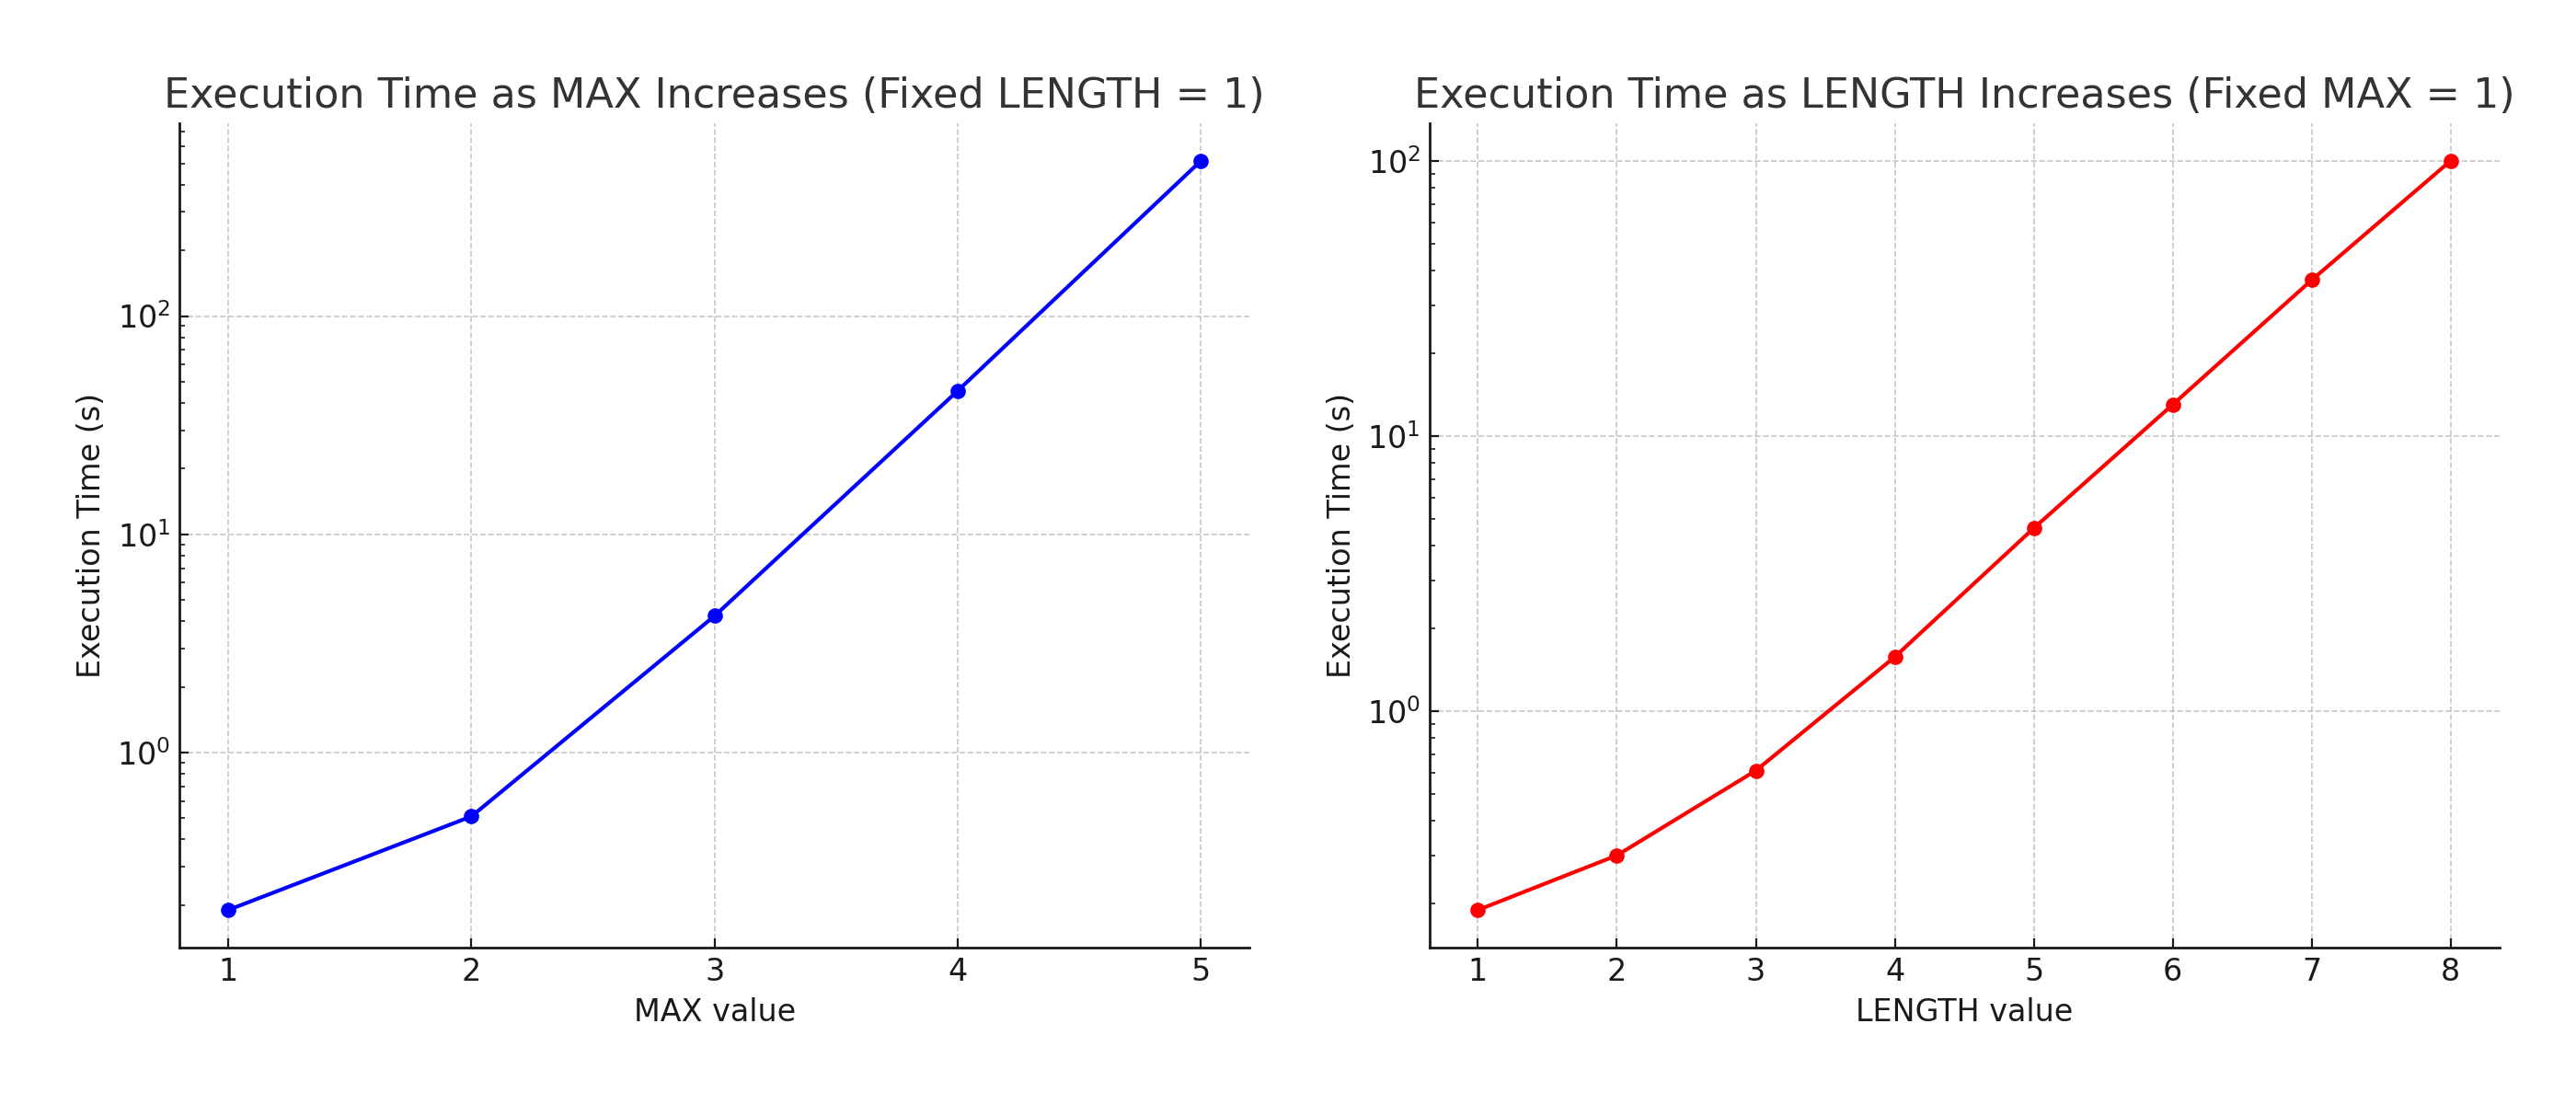
\includegraphics[width=1\textwidth]{./images/max_length_exec_time.png}
	\caption{Model checking execution time with different values of MAX and LENGTH}
	\label{fig:execution_time}
\end{figure}

Then, to have a better understanding, I also decided to increase the values of both MAX and LENGTH to understand how the model checking process behaves. Then, I merged the results in a single plot, available in figure \ref{fig:all_execution_time}.

\begin{figure}[H]
	\centering
	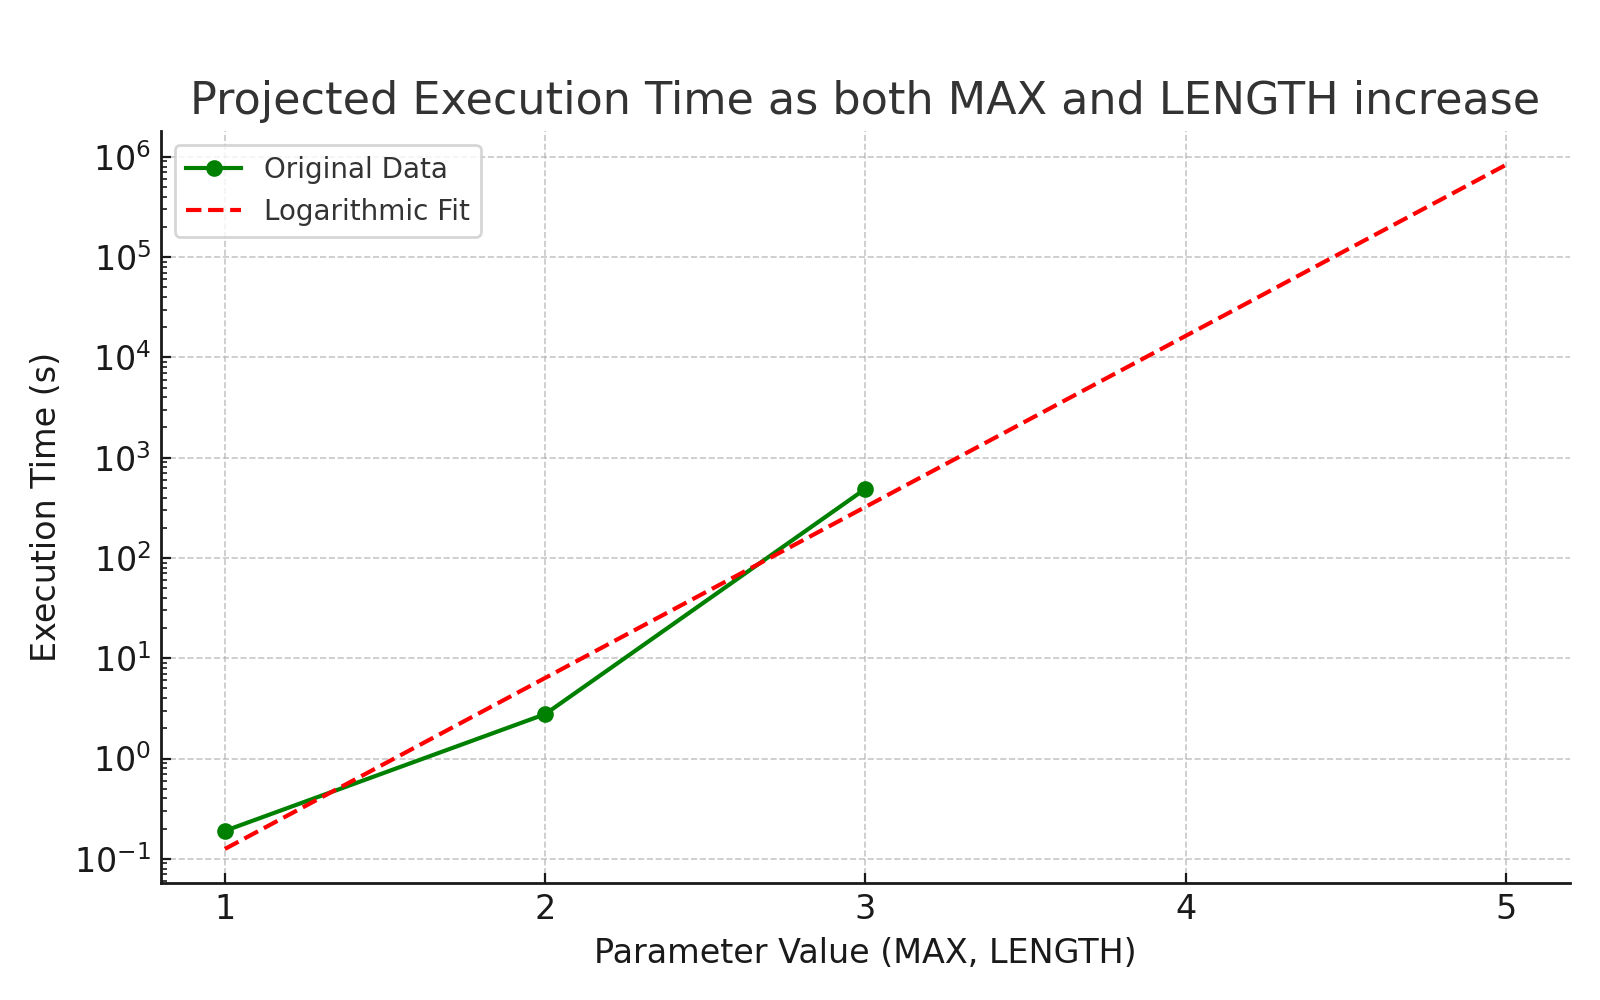
\includegraphics[width=0.9\textwidth]{./images/max_len_increase_exec_time.png}
	\caption{Model checking execution time with increasing values of MAX and LENGTH}
	\label{fig:all_execution_time}
\end{figure}

From the plot, it is possible to see that the model checking process is fast enough when the values of MAX and LENGTH are extremely low ($\leq 2$). However, as the values of MAX and LENGT increase, the model checking process becomes explonentially slower. This is expected, as the model checking process has to explore all possible states of the system, and the number of states grows exponentially with the values of MAX and LENGTH.

After the benchmarks outlined above, has been decided to set the valued of MAX and LENGTH to 2, to keep the model checking process fast and efficient enough to be able to analyze the behavior of the model.

\section{LTL Properties}

In the following subsections, I will discuss the LTL properties that have been defined to satisfy the requirements of the assignment. I developed

\subsection{Verify completition of both sequential and parallel processes}

To be able to verify the completition of both the sequential and parallel processes, I decided to use two global variables: \texttt{sequentialDone} and \texttt{parallelDone}. These variables are set to 0 by default, and set to 1 when the respective process has completed. To verify the completition of both processes, I defined the following LTL property:

\begin{lstlisting}[language=Promela, caption={LTL property to verify the completition of both sequential and parallel processes}, captionpos=b, breaklines=true]
ltl termination { <> (sequentialdone == 1 && paralleldone == 1) }
\end{lstlisting}

\subsection{Same most frequent value}
\label{sec:ltl_same_result}

To ensure that both versions of the frequency counter give the same result, I defined the following LTL property:

\begin{lstlisting}[language=Promela, caption={LTL property to verify that both versions of the frequency counter give the same result}]
ltl sameResult { [] (sequentialDone == 1 && parallelDone == 1) -> (sequential_result == parallel_result)}
\end{lstlisting}

This LTL verifies that the result of both versions (sequential and parallel) is the same after both processes have completed. This is important property to verify, as the two algorithms are expected to yield the same result.

\subsection{Sum of frequencies}

As we are interested in verifying the correctness of the frequency counter program, I decided to add an additional LTL properety that ensures that the sum of the frequencies of all values in the \texttt{sequential\_counts} and \texttt{parallel\_counts} arrays is equal to the length of the input array. This property is defined as follows:

\begin{lstlisting}[language=Promela, caption={LTL properties to verify the sum of frequencies in the sequential and parallel arrays}, captionpos=b, breaklines=true]
ltl sumCounts { [] (sequentialDone == 1 && parallelDone == 1) -> (sumCountsSequential == LENGTH && sumCountsParallel == LENGTH) }
\end{lstlisting}

As also possible to see from the code above, to verify this property I had to add two counters, \\ \texttt{sumCountsSequential} and \texttt{sumCountsParallel}, that are computed by summing the frequencies of all values in the respective arrays right before completing the respective processes. This way, I can verify that the sum of the frequencies is equal to the length of the input array.

\subsection{Invalid LTL formula: partial result}

As requesed by the assignment, I also added on purpose an invalid LTL formula that SPIN will not be able to verify. The property I decided to add is the following:

\begin{lstlisting}[language=Promela, caption={Invalid LTL property that SPIN will not be able to verify}, captionpos=b, breaklines=true]
ltl alwaysSameResult { [](sequential_result == parallel_result) }
\end{lstlisting}

This property is very similar to the \texttt{sameResult} property (refer to section \ref{sec:ltl_same_result}), but it does not take into account the completition of the processes. This LTL is wrong, as the two results are not expected to be the same while the processes are still running.

This is because the two versions of the program are not executed in parallel (first the sequential version and then the parallel version) and also, the two versions work in different ways. The sequential version computes the result and updates the \texttt{sequential\_result} variable as soon as it finds a value with a higher frequency. The parallel version, on the other hand, spawns multiple worker processes that concurrently compute the frequency of each value in the input array, and, only after all workers have completed, the main process updates the \texttt{parallel\_result} variable.

For these multiple reasons, the \texttt{alwaysSameResult} property is invalid and SPIN will find a counterexample right after the first iteration of the sequential process. This is the counterexample that SPIN will find (truncate for brevity):

\begin{lstlisting}
#processes: 2
                a[0] = 0
                a[1] = 0
                sequential_counts[0] = 1
                sequential_counts[1] = 0
                sequential_counts[2] = 0
                parallel_counts[0] = 0
                parallel_counts[1] = 0
                parallel_counts[2] = 0
                sequential_result = 0
                parallel_result = -1
                sequentialDone = 0
                parallelDone = 0
                sumCountsSequential = 0
                sumCountsParallel = 0
 41:    proc  1 (sequentialCounter:1) ../src/promela/model.pml:51 (state 12)
 41:    proc  0 (:init::1) ../src/promela/model.pml:42 (state 22)
 41:    proc  - (notSameResult:1) _spin_nvr.tmp:60 (state 6)
\end{lstlisting}

From the output above, it is possible to understand why, where and when SPIN found the counterexample: the LTL property is violated right after the first iteration of the sequential process as the two results are different ($sequential\_result = 0$ and $parallel\_result = -1$). At the moment ot the violation, the parallel process has not even started yet.

\section{Automatic SPIN verification via automation script}

To automate the verification process, has been created a script that will build the model, compile the resulting analyzer using \texttt{gcc}, and run the model checker using SPIN for each of the defined LTL properties. To run the script, it is possible to use the provided Makefile target "\texttt{run}" or run the script directly. Use the commands below to run the script:

\begin{lstlisting}
  make run
  # or
  ./scripts/run-model.sh
\end{lstlisting}

\end{document}
